\documentclass[10pt,a4paper]{article}

% ------------------------------------------------------------
% Page, font, and color setup
% ------------------------------------------------------------
\usepackage[a4paper,margin=2.05cm]{geometry}
\usepackage[utf8]{inputenc}
\usepackage[T1]{fontenc}
\usepackage[scaled=0.95]{helvet}
\renewcommand{\familydefault}{\sfdefault}
\usepackage{microtype}
\usepackage{ragged2e}
\usepackage{setspace}
\usepackage{array}
\usepackage{tabularx}
\usepackage{longtable}
\usepackage{booktabs}
\usepackage{enumitem}
\usepackage[table]{xcolor}
\usepackage{hyperref}
\usepackage{titlesec}
\usepackage{tcolorbox}
\tcbuselibrary{skins,breakable}
\usepackage{tikz}
\usetikzlibrary{arrows.meta,positioning,fit,calc,shapes.geometric,backgrounds}
\usepackage{fancyhdr}
\usepackage{lastpage}
\usepackage{caption}
\usepackage{float}
\usepackage{graphicx}
\usepackage{grffile}

\definecolor{navy}{HTML}{0D2D6E}
\definecolor{steel}{HTML}{1A3A6E}
\definecolor{accent}{HTML}{1565C0}
\definecolor{lightblue}{HTML}{E3F0FF}
\definecolor{paleblue}{HTML}{F4F9FF}
\definecolor{darkgrey}{HTML}{1F2937}
\definecolor{midgrey}{HTML}{374151}
\definecolor{lightgrey}{HTML}{F3F4F6}
\definecolor{linegrey}{HTML}{D1D5DB}
\definecolor{green}{HTML}{1B5E20}
\definecolor{greenlight}{HTML}{E8F5E9}
\definecolor{red}{HTML}{B71C1C}
\definecolor{redlight}{HTML}{FFEBEE}
\definecolor{purple}{HTML}{4A148C}
\definecolor{purplelight}{HTML}{F3E5F5}

\hypersetup{colorlinks=true,linkcolor=navy,urlcolor=accent,citecolor=navy}
\setlength{\parindent}{0pt}
\setlength{\parskip}{6pt}
\renewcommand{\arraystretch}{1.23}
\setlist[itemize]{leftmargin=*,topsep=3pt,itemsep=2pt,parsep=1pt}

% ------------------------------------------------------------
% Headers and section formatting
% ------------------------------------------------------------
\pagestyle{fancy}
\fancyhf{}
\lhead{\textcolor{midgrey}{Vendrai: Vendor-to-Pay Exception System}}
\rhead{\textcolor{midgrey}{NeuroX 1.0}}
\cfoot{\textcolor{midgrey}{Page \thepage\ of \pageref{LastPage}}}
\renewcommand{\headrulewidth}{0.3pt}
\renewcommand{\footrulewidth}{0pt}

\titleformat{\section}
  {\Large\bfseries\color{navy}}
  {\thesection}{0.7em}{}
\titlespacing*{\section}{0pt}{14pt}{8pt}

\newcommand{\sectionbanner}[2]{%
  \newpage
  \phantomsection
  \addcontentsline{toc}{section}{\protect\numberline{#1}#2}%
  \begin{tcolorbox}[colback=navy,colframe=navy,arc=0mm,boxrule=0pt,left=10pt,right=10pt,top=9pt,bottom=9pt]
    {\Large\bfseries\color{white}#1. #2}
  \end{tcolorbox}
}

\newcommand{\subhead}[1]{%
  \vspace{6pt}
  \phantomsection
  \addcontentsline{toc}{subsection}{#1}%
  {\large\bfseries\color{navy}#1}\par
  \vspace{-2pt}\textcolor{lightblue}{\rule{\linewidth}{1.1pt}}\vspace{2pt}
}

\newcommand{\minorhead}[1]{%
  \vspace{4pt}
  {\normalsize\bfseries\color{accent}#1}\par
}

\newtcolorbox{callout}[2][]{
  colback=#2,
  colframe=#2,
  borderline west={3pt}{0pt}{accent},
  boxrule=0pt,
  arc=0mm,
  left=9pt,right=9pt,top=8pt,bottom=8pt,
  #1
}

\newtcolorbox{safetybox}{
  colback=redlight,
  colframe=redlight,
  borderline west={3pt}{0pt}{red},
  boxrule=0pt,
  arc=0mm,
  left=9pt,right=9pt,top=8pt,bottom=8pt
}

\newtcolorbox{greenbox}{
  colback=greenlight,
  colframe=greenlight,
  borderline west={3pt}{0pt}{green},
  boxrule=0pt,
  arc=0mm,
  left=9pt,right=9pt,top=8pt,bottom=8pt
}

\newcolumntype{Y}{>{\RaggedRight\arraybackslash}X}
\newcolumntype{C}[1]{>{\centering\arraybackslash}p{#1}}
\newcolumntype{L}[1]{>{\RaggedRight\arraybackslash}p{#1}}

\newcommand{\tableheader}[1]{\textbf{\color{white}#1}}
\newcommand{\smalltext}[1]{{\small #1}}

% ------------------------------------------------------------
% TikZ styles
% ------------------------------------------------------------
\tikzset{
  layerbox/.style={rectangle,rounded corners=2pt,draw=navy,thick,fill=lightblue,align=center,text width=3.0cm,minimum height=1.0cm,font=\small\bfseries},
  toolbox/.style={rectangle,rounded corners=2pt,draw=steel,thick,fill=lightgrey,align=center,text width=2.75cm,minimum height=0.95cm,font=\scriptsize},
  agentbox/.style={rectangle,rounded corners=2pt,draw=navy,thick,fill=paleblue,align=center,text width=2.45cm,minimum height=0.9cm,font=\scriptsize\bfseries},
  statebox/.style={rectangle,rounded corners=2pt,draw=green,thick,fill=greenlight,align=center,text width=2.8cm,minimum height=0.95cm,font=\scriptsize\bfseries},
  hitlbox/.style={rectangle,rounded corners=2pt,draw=red,thick,fill=redlight,align=center,text width=3.0cm,minimum height=0.95cm,font=\scriptsize\bfseries},
  arrow/.style={-{Latex[length=2.2mm]},thick,draw=midgrey},
  dasharrow/.style={-{Latex[length=2.2mm]},thick,dashed,draw=midgrey}
}

\begin{document}

% ------------------------------------------------------------
% Cover page
% ------------------------------------------------------------
\thispagestyle{empty}
\vspace*{0.4cm}
\begin{tcolorbox}[colback=navy,colframe=navy,boxrule=0pt,arc=0mm,left=12pt,right=12pt,top=30pt,bottom=30pt,width=\linewidth]
  \centering
  {\fontsize{27}{34}\selectfont\bfseries\color{white}Vendrai\\[3pt]Vendor-to-Pay Exception System}
\end{tcolorbox}

\vspace{0.6cm}
\begin{tcolorbox}[colback=steel,colframe=steel,boxrule=0pt,arc=0mm,left=12pt,right=12pt,top=18pt,bottom=18pt,width=\linewidth]
  \centering
  {\Large\color{lightblue}Parallel Multi-Agent B2B Agentic Workflow\\[4pt]for Procurement and Finance Operations}
\end{tcolorbox}

\vspace{1.0cm}
\begin{tabularx}{\linewidth}{>{\bfseries\color{navy}}L{3.7cm}Y}
\rowcolor{lightgrey}
Competition & NeuroX 1.0 - National Level Buildathon \\
\rowcolor{lightgrey}
Track & B2B Agentic AI - Financial Operations \& Procurement \\
\rowcolor{lightgrey}
Phase & Phase 1: Idea Validation \\
\rowcolor{lightgrey}
Submitted by & Gmora \\
\rowcolor{lightgrey}
Submitted & July 12, 2026 \\
\end{tabularx}

\vfill
\begin{center}
\textcolor{midgrey}{Detailed Report - Problem Statement, Value Proposition, Agentic Loop, Architecture, Tool Mapping, and HITL Design}
\end{center}
\newpage

\tableofcontents
\newpage

% ------------------------------------------------------------
% 1. Problem Statement
% ------------------------------------------------------------
\sectionbanner{1}{Problem Statement}

\begin{callout}{lightblue}
\textbf{The problem identified:} In medium and large B2B organisations, the Vendor-to-Pay workflow - spanning supplier onboarding through invoice exception resolution - remains one of the most manual, repetitive, and judgement-intensive operational bottlenecks in procurement and finance. The workflow is not blocked by a lack of forms or databases; it is blocked by the gap between messy business evidence and ERP-ready decisions.
\end{callout}

\subhead{1.1 The Operational Reality}
When a business department needs to engage a new supplier, a procurement analyst must collect and cross-verify multiple documents: tax certificates, bank letters, insurance certificates, contracts, supplier questionnaires, and sometimes security or compliance forms. These documents arrive through email threads, shared folders, procurement portals, or direct uploads, and they rarely follow one standard format. The same supplier may appear under different trading names in different documents. A bank letter may use a legal name while a tax certificate uses a registered business name. The requester may describe the supplier as a general service vendor even though the supplier provides software access, which changes the approval path entirely.

Even after documents are collected, the analyst must decide whether the vendor already exists in the ERP under a similar name, whether the supplier category is correct, whether all documents are present, whether policy approvals have been triggered, and whether the data is clean enough to create a vendor master record. This work is repetitive, but it still requires judgement. The analyst is not just filling fields; the analyst is interpreting evidence, resolving contradictions, and deciding what should happen next.

\subhead{1.2 The Invoice Exception Problem}
The same bottleneck appears downstream in accounts payable. When an invoice does not automatically match a purchase order or goods receipt note, the AP specialist must manually investigate the mismatch type. The issue may be a price variance, quantity discrepancy, missing PO reference, incorrect tax amount, duplicate invoice number, wrong vendor code, currency mismatch, or vendor name mismatch. Each exception requires a different investigation path and different evidence.

For example, a price variance may require contract or procurement approval, while a quantity discrepancy may require warehouse confirmation. A bank detail mismatch may require finance risk review, and a duplicate invoice warning may require historical invoice search. AP teams therefore spend significant time chasing information across procurement teams, warehouse users, vendor contacts, ERP records, and email chains before they can recommend a resolution.

\subhead{1.3 Why Existing Tools Fail}
ERP systems, procurement suites, AP automation tools, and rule-based workflow engines already exist, but they do not solve the full operational problem. ERP systems store vendor and invoice data, but they do not reliably interpret inconsistent external documents. Procurement platforms can route structured approvals, but they depend on humans to enter clean and validated data. AP automation systems can detect exceptions, but they often leave humans with large exception queues that still require manual investigation.

Rule-based workflow engines are useful when the process is predictable: if spend is above a threshold, route to a manager; if the invoice total differs from the PO total, flag an exception. However, the difficult cases are not that simple. The system must understand uncertain OCR output, conflicting supplier names, missing documents, risk API failures, ambiguous policy rules, and incomplete requester information. A simple chatbot also does not solve this because the task is not conversation alone. The task is a stateful investigation across multiple tools, documents, policies, and approvals.

\begin{greenbox}
The result is a workflow that is repetitive enough to be worth automating, but judgement-intensive enough to have resisted traditional automation. This is exactly the class of B2B workflow where agentic AI can create value: the agent can collect evidence, select tools, reason about uncertainty, recover from failures, and prepare an accountable recommendation while preserving human control over high-risk execution.
\end{greenbox}

% ------------------------------------------------------------
% 2. Value Proposition
% ------------------------------------------------------------
\sectionbanner{2}{Value Proposition}

\subhead{2.1 Why This Problem Is Worth Solving}
Vendor-to-Pay operations affect cash flow, procurement speed, supplier relationships, fraud exposure, and financial control. Slow supplier onboarding delays project starts and frustrates internal requesters. Unresolved invoice exceptions delay payments, damage supplier relationships, and consume AP team capacity. Duplicate or inconsistent vendor master records create payment errors, compliance failures, and audit difficulties. These are not rare edge cases; they are daily operational realities in B2B organisations with active procurement and finance teams.

The business willingness to pay for this type of solution is realistic because the cost is measurable. Enterprises already spend heavily on ERP systems, procurement platforms, AP automation, vendor risk tools, and compliance tooling. A system that reduces onboarding cycle time, improves vendor master quality, shortens AP investigation time, and produces audit-ready evidence can be justified through productivity savings, reduced rework, faster cycle times, and lower operational risk.

\subhead{2.2 How an Agentic Workflow Improves on Manual Practice}
\begin{table}[H]
\centering
\small
\begin{tabularx}{\linewidth}{L{2.8cm}Y Y}
\rowcolor{navy}
\tableheader{Dimension} & \tableheader{Current Manual Practice} & \tableheader{Proposed Agentic System} \\
\rowcolor{lightblue}
Speed & Sequential investigation through emails, ERP screens, and shared folders. & Multiple independent checks are launched together; the agent waits only where a real dependency exists. \\
\rowcolor{lightgrey}
Consistency & Analyst-dependent checks; important evidence may be missed during busy periods. & The same policy checklist, risk checks, and evidence requirements are applied to every case. \\
\rowcolor{lightblue}
Ambiguity & Escalation depends on individual judgement and may be ad hoc. & Confidence thresholds and contradiction rules trigger targeted clarification or human review. \\
\rowcolor{lightgrey}
Error recovery & Failed checks may be retried manually or silently skipped. & Tool calls return structured results; failures trigger retry, pending state, or escalation. \\
\rowcolor{lightblue}
Auditability & Evidence is scattered across emails, spreadsheets, and ERP notes. & Every agent action, tool call, recommendation, and human decision is logged centrally. \\
\rowcolor{lightgrey}
Scalability & Throughput increases mainly by adding more analysts. & Investigation work scales with automation while humans focus on approval and exception judgement. \\
\end{tabularx}
\caption{Operational improvement from manual Vendor-to-Pay work to an agentic investigation workflow.}
\end{table}

\subhead{2.3 Why Agentic AI Is Better Than Traditional Software Here}
The value of this system is not simply that an LLM is connected to enterprise tools. The value is that the system can maintain case state, compare evidence from multiple sources, decide which tool should be called next, and change its route when the case becomes ambiguous. Traditional software is excellent when the process is fixed and the input is structured. This workflow is different: documents are inconsistent, data is incomplete, policies depend on context, and external tools may fail.

The proposed system uses automation for the repetitive investigation work and agentic reasoning for the judgement-heavy parts that traditional software struggles with. It does not replace the human in high-risk decisions. Instead, it prepares a complete, evidence-backed decision packet so that human reviewers can make faster and more reliable decisions. This combination of agentic investigation and human-controlled execution creates the practical enterprise value.

% ------------------------------------------------------------
% 3. Proposed Autonomous Agent Solution
% ------------------------------------------------------------
\sectionbanner{3}{Proposed Autonomous Agent Solution}

\begin{callout}{lightblue}
\textbf{Core design principle:} The system uses a parallel multi-agent pattern where specialist agents investigate different parts of the case and write their results into a shared state. Parallelism is important because supplier documents, duplicate checks, risk checks, and policy retrieval can be investigated independently. However, the main strength is not parallelism alone; it is the combination of parallel evidence collection, shared state, dynamic reasoning, structured error recovery, and human approval before risky execution.
\end{callout}

\subhead{3.1 System Overview}
The Vendrai system operates as an intelligent case management platform for supplier onboarding and AP invoice exception handling. A case may begin from a web form, email trigger, ERP event, or document upload. The Supervisor Agent first classifies the case and initializes the investigation state. It then launches the relevant specialist agents, such as Document Extraction, Duplicate Detection, Risk Checking, and Policy Retrieval. These agents operate independently where possible and write their findings into a shared annotated state.

After the specialist outputs are available, the Reasoning Agent reads the combined evidence. It decides whether the case is clean enough to proceed, whether a missing document must be requested, whether a possible duplicate requires human review, whether a risk flag changes the approval route, or whether a tool failure blocks the case. The loop continues until the Verifier Agent confirms that the recommendation is complete, evidence-based, and safe to send to the human approval queue.

\subhead{3.2 Multi-Agent Design Without Overclaiming}
This proposal deliberately avoids the common mistake of naming every function an agent. Each agent has a clear responsibility, a limited tool set, and a measurable output. The Document Agent extracts fields and confidence scores. The Duplicate Agent searches for similar vendors. The Risk Agent checks sanctions and fraud signals. The Policy Agent retrieves relevant approval rules. The Reasoning Agent interprets all outputs together and decides the next action. This design keeps the system modular and testable.

Parallel execution is used when it improves speed and does not create unsafe dependencies. For example, OCR extraction, vendor master search, risk checking, and policy retrieval can be launched in the same investigation round. The system does not claim that every step must be parallel. Some steps must remain sequential for safety, such as waiting for human duplicate review before ERP sync. This balanced design is more credible than simply saying everything runs in parallel.

\subhead{3.3 Agent Roster and Responsibilities}
\begin{longtable}{L{3.3cm}L{7.0cm}L{4.3cm}}
\rowcolor{navy}
\tableheader{Agent} & \tableheader{Role} & \tableheader{Main Tools Used} \\
\endfirsthead
\rowcolor{navy}
\tableheader{Agent} & \tableheader{Role} & \tableheader{Main Tools Used} \\
\endhead
\rowcolor{lightblue}
Supervisor Agent & Orchestrates the workflow, identifies case type, initializes state, launches specialist agents, and monitors completion. & Case database, routing logic, LangGraph graph state \\
\rowcolor{lightgrey}
Document Agent & Extracts structured fields from supplier documents and invoices, including confidence scores and source references. & Free-tier OCR API, field normalizer, document store \\
\rowcolor{lightblue}
Duplicate Detection Agent & Searches the vendor master for similar records using legal name, trading name, tax ID, address, and bank account signals. & ERP vendor master API, similarity engine, fuzzy search \\
\rowcolor{lightgrey}
Risk Agent & Checks sanctions, PEP exposure, bank country mismatch, adverse signals, and other supplier risk indicators. & Sanctions/risk API, bank risk data, vendor profile data \\
\rowcolor{lightblue}
Policy Agent & Retrieves applicable procurement, AP, risk, and approval policies based on vendor category, spend level, region, and exception type. & Qdrant knowledge base, policy database \\
\rowcolor{lightgrey}
Reasoning Agent & Reads all current evidence, identifies gaps and conflicts, classifies case risk, and chooses the next action dynamically. & Shared state, LLM, structured routing schema \\
\rowcolor{lightblue}
Clarification Agent & Drafts targeted clarification requests when missing or ambiguous information blocks the next decision. & Email API, Slack or Teams API, message templates \\
\rowcolor{lightgrey}
Retry Agent & Handles failed or unavailable tools using retry policies, backoff, pending state, and escalation. & Tool gateway, retry scheduler, audit log \\
\rowcolor{lightblue}
Evidence Builder Agent & Builds the human approval packet with recommendation, reasoning summary, extracted fields, confidence scores, and evidence links. & Shared state, document store, approval queue API \\
\rowcolor{lightgrey}
Verifier Agent & Checks that mandatory fields are present, risk checks are complete, evidence supports the recommendation, and no unsafe action is proposed. & Policy rules, safety checklist, audit schema \\
\rowcolor{lightblue}
ERP Sync Agent & After human approval only, proposes or confirms vendor creation or invoice resolution in the ERP or accounting system. & ERP/accounting API, approval result, audit log \\
\caption{Agent roster with clear responsibilities and tool boundaries.}
\end{longtable}

% ------------------------------------------------------------
% 4. Agentic Loop
% ------------------------------------------------------------
\sectionbanner{4}{Proposed Agentic Loop}

\subhead{4.1 Core Loop Structure}
The agentic loop begins when a new case enters the system. The Supervisor Agent reads the case payload, including requester details, uploaded documents, invoice metadata, supplier category, and current case type. It then creates an initial state object and launches the relevant specialist agents. In the normal supplier onboarding flow, the first investigation round includes document extraction, duplicate detection, risk checking, and policy retrieval. Each agent calls its own tools and writes structured output back to the shared state.

The Reasoning Agent is activated after the first investigation round. It does not follow a rigid decision tree. It evaluates the combined evidence and asks questions such as: Are required documents missing? Are extracted fields reliable enough? Is there a possible duplicate vendor? Did a risk tool fail? Does the policy require legal, finance, or security approval? Does any recommendation depend on unresolved evidence? Based on those answers, it chooses the next action: continue, request clarification, retry a tool, route to human duplicate review, build an approval packet, or escalate the case.

\begin{figure}[H]
\centering
\resizebox{\linewidth}{!}{%
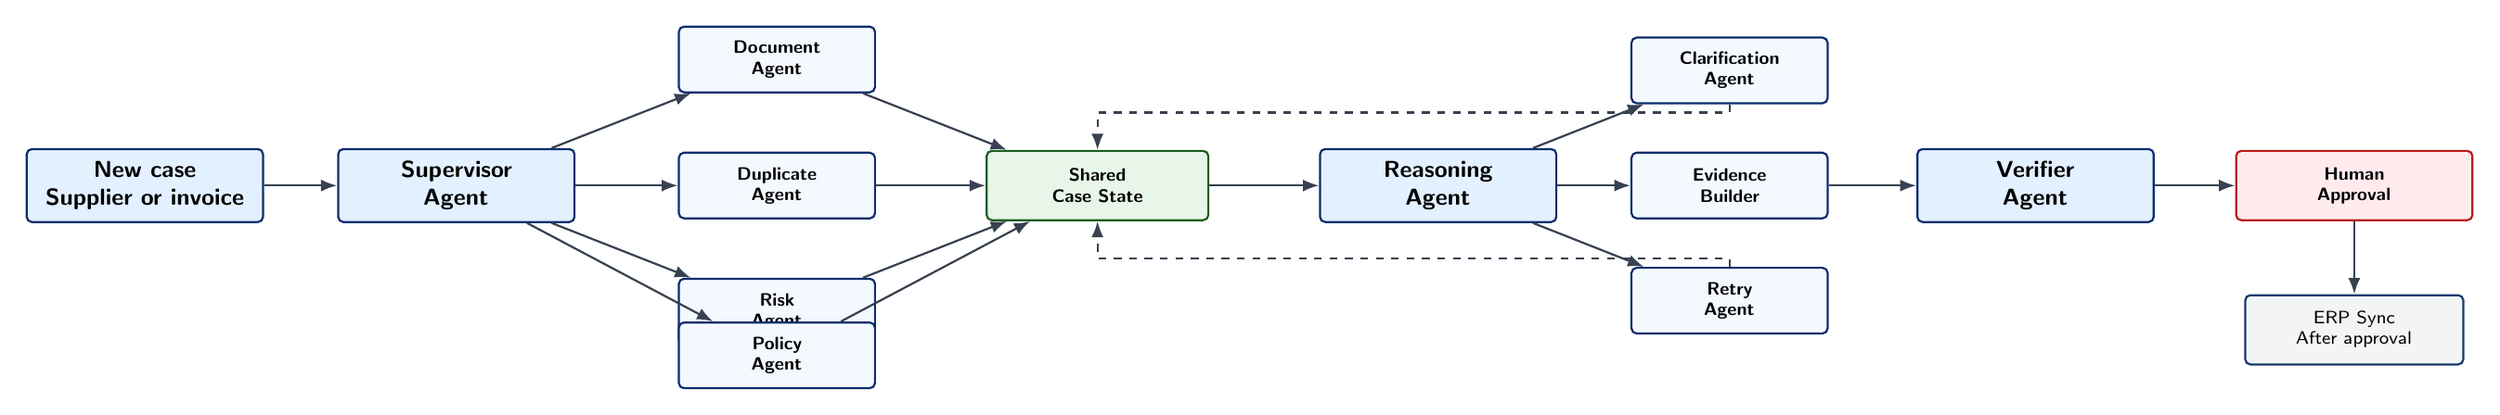
\begin{tikzpicture}[node distance=1.0cm and 1.0cm]
  \node[layerbox] (case) {New case\\Supplier or invoice};
  \node[layerbox, right=of case] (sup) {Supervisor\\Agent};
  \node[agentbox, above right=0.75cm and 1.4cm of sup] (doc) {Document\\Agent};
  \node[agentbox, right=1.4cm of sup] (dup) {Duplicate\\Agent};
  \node[agentbox, below right=0.75cm and 1.4cm of sup] (risk) {Risk\\Agent};
  \node[agentbox, below=1.4cm of dup] (pol) {Policy\\Agent};
  \node[statebox, right=1.5cm of dup] (state) {Shared\\Case State};
  \node[layerbox, right=1.5cm of state] (reason) {Reasoning\\Agent};
  \node[agentbox, above right=0.6cm and 1.0cm of reason] (clar) {Clarification\\Agent};
  \node[agentbox, right=1.0cm of reason] (evid) {Evidence\\Builder};
  \node[agentbox, below right=0.6cm and 1.0cm of reason] (retry) {Retry\\Agent};
  \node[layerbox, right=1.2cm of evid] (ver) {Verifier\\Agent};
  \node[hitlbox, right=1.1cm of ver] (human) {Human\\Approval};
  \node[toolbox, below=1.0cm of human] (erp) {ERP Sync\\After approval};

  \draw[arrow] (case) -- (sup);
  \draw[arrow] (sup) -- (doc);
  \draw[arrow] (sup) -- (dup);
  \draw[arrow] (sup) -- (risk);
  \draw[arrow] (sup) -- (pol);
  \draw[arrow] (doc) -- (state);
  \draw[arrow] (dup) -- (state);
  \draw[arrow] (risk) -- (state);
  \draw[arrow] (pol) -- (state);
  \draw[arrow] (state) -- (reason);
  \draw[arrow] (reason) -- (clar);
  \draw[arrow] (reason) -- (evid);
  \draw[arrow] (reason) -- (retry);
  \draw[arrow] (evid) -- (ver);
  \draw[arrow] (ver) -- (human);
  \draw[arrow] (human) -- (erp);
  \draw[dasharrow] (clar) |- ($(state)+(0,1.0)$) -- (state);
  \draw[dasharrow] (retry) |- ($(state)+(0,-1.0)$) -- (state);
\end{tikzpicture}}
\caption{Agentic loop: independent evidence collection, shared state, dynamic reasoning, verification, and human approval before execution.}
\end{figure}

\subhead{4.2 Dynamic Reasoning and Decision-Making}
The decision path changes depending on the case. A clean low-risk supplier with complete documents, no duplicate match, and spend below threshold can move quickly to evidence building and a single procurement approval. A software supplier that may access customer data causes the Policy Agent to retrieve security review requirements, and the Reasoning Agent adds IT security approval to the packet. A supplier whose bank account country differs from the registered country causes the Risk Agent to flag the case, and the Reasoning Agent adds finance review. A possible duplicate pauses the loop and creates a human duplicate resolution task before the case can proceed.

The important point is that the agent does not merely execute a predefined checklist. It uses the current state of the case to decide what to do next. It can re-run a failed risk check, ask for a missing bank letter, request a clearer tax certificate, retrieve additional policy sections, or escalate the case to a human reviewer. This dynamic behaviour is what separates the system from a linear automation script.

\subhead{4.3 Ambiguous Input Handling}
Ambiguity is expected in Vendor-to-Pay workflows. The system therefore handles ambiguity through confidence thresholds and explicit contradiction handling. High-confidence extracted fields, such as fields above 90 percent confidence, can be used directly in the evidence packet. Medium-confidence fields are shown to the reviewer with their confidence score and source reference. Low-confidence fields trigger the Clarification Agent to request a better document or a direct confirmation from the requester or vendor.

Contradictory evidence is not hidden. If the supplier name on a tax certificate does not match the supplier name on the bank letter, the Reasoning Agent flags the contradiction and asks for resolution. If the vendor category is unclear, the agent asks a targeted question instead of guessing, because category affects risk review and approval route. If the duplicate score is high but not conclusive, the system pauses for human duplicate review rather than merging records autonomously.

\subhead{4.4 Tool Error Recovery}
The system treats tool failures as normal operational events. Every external call goes through a Tool Gateway that validates input, checks permissions, calls the external tool, captures the response, and returns a structured result. The Reasoning Agent must explicitly evaluate each result. The system never pretends that a check passed when the tool failed.

\begin{table}[H]
\centering
\small
\begin{tabularx}{\linewidth}{L{4.3cm}Y}
\rowcolor{navy}
\tableheader{Error Type} & \tableheader{Recovery Action} \\
\rowcolor{redlight}
API timeout & Retry with exponential backoff up to a defined limit, then mark the check as pending and continue only if policy allows. \\
\rowcolor{lightgrey}
Low-confidence OCR & Request a clearer document or direct field confirmation from the vendor or requester. \\
\rowcolor{redlight}
Ambiguous ERP search & Route to human duplicate review before allowing vendor creation or duplicate merge. \\
\rowcolor{lightgrey}
Risk API unavailable & Mark risk check as pending and block final approval until the check completes or a human override is explicitly recorded. \\
\rowcolor{redlight}
Permission denied on ERP write & Route to an authorised user and record the failure; do not retry autonomously with different permissions. \\
\rowcolor{lightgrey}
Conflicting policy retrieval & Escalate to compliance or procurement policy owner instead of inventing a resolution. \\
\rowcolor{redlight}
Email delivery failure & Retry through an alternate channel such as Slack or Teams and log the failed delivery. \\
\end{tabularx}
\caption{Structured recovery logic for external tool failures.}
\end{table}

\begin{safetybox}
\textbf{Critical safety rule:} The agent never assumes that an ERP write succeeded unless the ERP confirms it. It never marks a case complete when required evidence is missing. It never claims a risk check passed if the risk tool failed. This makes silent failure architecturally visible rather than hidden.
\end{safetybox}

% ------------------------------------------------------------
% 5. Architecture and Tool Mapping
% ------------------------------------------------------------
\sectionbanner{5}{Architecture and Tool Mapping}

\subhead{5.1 System Architecture Layers}
The architecture is separated into presentation, core backend, agent runtime, tool gateway, and knowledge/data layers. This separation makes the system modular and easier to test. The core backend owns users, cases, approvals, and audit logs. The agent runtime owns reasoning and state transitions. The tool gateway owns external tool access and error normalization. The knowledge layer stores policies, documents, embeddings, and case memory.

\begin{figure}[H]
\centering
\resizebox{\linewidth}{!}{%
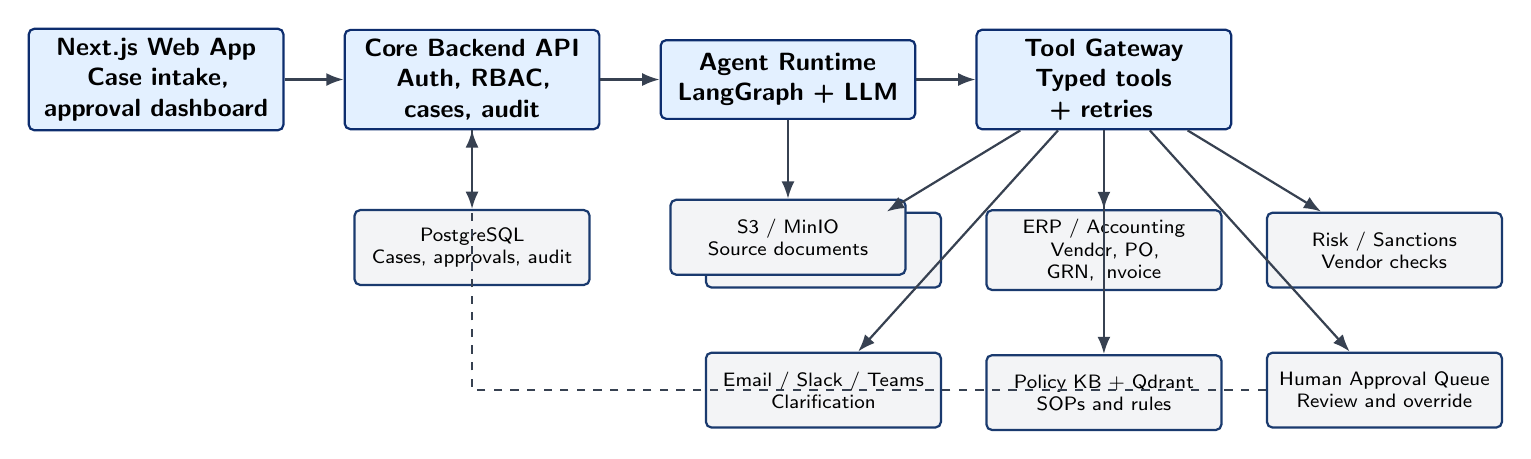
\begin{tikzpicture}[node distance=0.95cm and 0.75cm]
  \node[layerbox] (ui) {Next.js Web App\\Case intake, approval dashboard};
  \node[layerbox, right=of ui] (api) {Core Backend API\\Auth, RBAC, cases, audit};
  \node[layerbox, right=of api] (agent) {Agent Runtime\\LangGraph + LLM};
  \node[layerbox, right=of agent] (gateway) {Tool Gateway\\Typed tools + retries};

  \node[toolbox, below=1.0cm of gateway] (erp) {ERP / Accounting\\Vendor, PO, GRN, invoice};
  \node[toolbox, left=0.55cm of erp] (ocr) {Free-tier OCR API\\PDF extraction};
  \node[toolbox, right=0.55cm of erp] (risk) {Risk / Sanctions\\Vendor checks};
  \node[toolbox, below=0.8cm of ocr] (email) {Email / Slack / Teams\\Clarification};
  \node[toolbox, below=0.8cm of erp] (vector) {Policy KB + Qdrant\\SOPs and rules};
  \node[toolbox, below=0.8cm of risk] (hitl) {Human Approval Queue\\Review and override};

  \node[toolbox, below=1.0cm of api] (db) {PostgreSQL\\Cases, approvals, audit};
  \node[toolbox, below=1.0cm of agent] (store) {S3 / MinIO\\Source documents};

  \draw[arrow] (ui) -- (api);
  \draw[arrow] (api) -- (agent);
  \draw[arrow] (agent) -- (gateway);
  \draw[arrow] (api) -- (db);
  \draw[arrow] (agent) -- (store);
  \draw[arrow] (gateway) -- (ocr);
  \draw[arrow] (gateway) -- (erp);
  \draw[arrow] (gateway) -- (risk);
  \draw[arrow] (gateway) -- (email);
  \draw[arrow] (gateway) -- (vector);
  \draw[arrow] (gateway) -- (hitl);
  \draw[dasharrow] (hitl) -| (api);
\end{tikzpicture}}
\caption{Technical architecture with external tools and data sources selected by the agent through a controlled tool gateway.}
\end{figure}

\begin{figure}[H]
\centering

\includegraphics[width=\linewidth]{System Architecture Diagram.png}
\caption{System Architecture Diagram}
\end{figure}

\begin{figure}[H]
\centering

\includegraphics[width=\linewidth]{ER diagram.png}
\caption{Entity-Relationship (ER) Diagram}
\end{figure}

\begin{table}[H]
\centering
\small
\begin{tabularx}{\linewidth}{L{3.2cm}L{4.5cm}Y}
\rowcolor{navy}
\tableheader{Layer} & \tableheader{Components} & \tableheader{Responsibility} \\
\rowcolor{lightblue}
Presentation & Next.js web app, React dashboard & Case intake, document upload, recommendation display, approval queue, document viewer, audit view. \\
\rowcolor{lightgrey}
Core Backend & FastAPI, PostgreSQL, Redis & Authentication, RBAC, case records, approval states, background jobs, audit logs, integration credentials. \\
\rowcolor{lightblue}
Agent Runtime & LangGraph, Python, LLM provider & Supervisor orchestration, stateful reasoning loop, specialist agent execution, dynamic routing. \\
\rowcolor{lightgrey}
Tool Gateway & Typed tool functions, validation layer & Input validation, permission checks, structured responses, retry logic, and audit logging for every call. \\
\rowcolor{lightblue}
Knowledge and Data & Qdrant (Vector DB), PostgreSQL + pgvector (Primary DB), S3 & Policy embeddings, vendor records, invoice records, document storage, approved case memory. \\
\end{tabularx}
\caption{Layered system architecture and responsibilities.}
\end{table}

\subhead{5.2 Architecture Flow Specification}
A user creates a case through the web application. The backend stores the case and triggers the agent runtime. The Supervisor Agent selects the initial investigation path. Specialist agents call tools through the Tool Gateway and write results into shared state. The Reasoning Agent evaluates the results and chooses whether to clarify, retry, escalate, or build the evidence packet. The Verifier Agent checks safety and completeness. The human reviewer then approves, edits, rejects, redirects, or escalates. Only after approval can the ERP Sync Agent propose or execute an approved update in the ERP or accounting system.

\begin{figure}[H]
\centering

\includegraphics[width=\linewidth]{Vendor Onboarding Flow diagram.png}
\caption{Vendor Onboarding Flow Diagram}
\end{figure}

\begin{figure}[H]
\centering

\includegraphics[width=\linewidth]{Invoice Exception Resolution Workflow diagram.png}
\caption{Invoice Exception Resolution Workflow Diagram}
\end{figure}

\subhead{5.3 External Tool and API Mapping}
\begin{longtable}{L{3.3cm}L{4.3cm}L{5.1cm}L{2.5cm}}
\rowcolor{navy}
\tableheader{Tool / API} & \tableheader{Purpose in Workflow} & \tableheader{Dynamic Use by Agent} & \tableheader{Called By} \\
\endfirsthead
\rowcolor{navy}
\tableheader{Tool / API} & \tableheader{Purpose in Workflow} & \tableheader{Dynamic Use by Agent} & \tableheader{Called By} \\
\endhead
\rowcolor{lightblue}
Free-tier OCR API & Extracts structured fields from invoices, tax certificates, bank letters, contracts, and supplier questionnaires. & Selected when documents are uploaded. Confidence scores determine whether the field is accepted, shown for confirmation, or sent for clarification. & Document Agent \\
\rowcolor{lightgrey}
ERP / Accounting System API & Provides vendor master data, PO records, goods receipts, invoice history, and approved write endpoints. & Used for duplicate search, PO/GRN retrieval, invoice matching, and approved ERP sync only after HITL approval. & Duplicate Agent, Reasoning Agent, ERP Sync Agent \\
\rowcolor{lightblue}
Vendor Risk / Sanctions API & Checks sanctions, PEP exposure, bank country risk, fraud signals, and adverse supplier indicators. & Called for new supplier cases. If unavailable, the risk check is marked pending and final approval is blocked or escalated. & Risk Agent \\
\rowcolor{lightgrey}
Email / Slack / Teams API & Sends targeted clarification requests to requesters, vendors, or internal reviewers. & Used only when the next decision depends on missing or ambiguous information. The message is specific to the blocking issue. & Clarification Agent \\
\rowcolor{lightblue}
Policy Knowledge Base & Stores procurement policies, AP policies, approval matrices, SOPs, and past approved case summaries. & Retrieved semantically using Qdrant. The Reasoning Agent uses retrieved policy evidence before routing approval decisions. & Policy Agent \\
\rowcolor{lightgrey}
Human Approval Queue & Provides structured review tasks with evidence packets and authorized decision controls. & Created after verification. ERP sync remains blocked until the approval queue returns an approved status. & Evidence Builder, Verifier, ERP Sync Agent \\
\caption{External tools and data sources integrated into the agent reasoning loop.}
\end{longtable}

% ------------------------------------------------------------
% 6. Human-in-the-Loop Design
% ------------------------------------------------------------
\sectionbanner{6}{Human-in-the-Loop (HITL) Design}

\begin{callout}{lightblue}
\textbf{Design philosophy:} Human oversight is placed where business risk, legal accountability, financial exposure, or policy ambiguity is highest. The agent automates investigation; humans authorize execution.
\end{callout}

\subhead{6.1 Primary Control Point: The Approval Packet}
The central HITL mechanism is the structured approval packet. The Evidence Builder Agent produces this packet only after investigation, and the Verifier Agent checks it before it reaches a reviewer. The packet includes the recommended action, reasoning summary, extracted fields with confidence scores, risk assessment results, policy requirements, source document links, tool call results, unresolved ambiguities, and the exact approval action required.

The human reviewer can approve the recommendation, edit extracted fields or the recommendation, request more information, reject the case, or escalate it to a senior reviewer or different department. This control point occurs before execution, not after. No ERP write, vendor creation, duplicate merge, invoice exception approval, or bank detail change occurs without human approval.

\subhead{6.2 What the Agent Can Do Without Approval}
The agent can read case data, process uploaded documents, call OCR tools, search the vendor master, retrieve purchase orders and goods receipts, perform duplicate detection, run risk checks, retrieve policies, compare invoice lines against PO and GRN data, classify exception types, draft clarification messages, build evidence packets, and create approval tasks. These actions are logged, but they do not require pre-approval because they do not change a financial record or create a business commitment.

\subhead{6.3 Actions That Always Require Human Approval}
Creating a new vendor record, changing vendor bank details, merging vendor records, rejecting supplier onboarding, approving invoice exceptions above tolerance, overriding failed or pending risk checks, modifying approved policy knowledge, or performing any payment-related action requires human approval. This is not a cosmetic control. It is a hard execution gate in the workflow.

\begin{table}[H]
\centering
\small
\begin{tabularx}{\linewidth}{L{4.5cm}Y L{3.3cm}}
\rowcolor{navy}
\tableheader{Action} & \tableheader{Reason for Control} & \tableheader{Human Decision} \\
\rowcolor{redlight}
Create vendor in ERP & Creates a new financial trading relationship and affects procurement/payment systems. & Approve, edit, reject \\
\rowcolor{lightgrey}
Change bank details & High fraud and payment redirection risk. & Approve only after evidence review \\
\rowcolor{redlight}
Merge duplicate vendors & Incorrect merge can corrupt vendor master and payment history. & Merge, reject match, continue new \\
\rowcolor{lightgrey}
Approve invoice exception above tolerance & Financial accountability and possible policy override. & Approve, escalate, reject \\
\rowcolor{redlight}
Override failed risk check & Compliance and audit responsibility. & Escalate or document exception \\
\end{tabularx}
\caption{Human approval gates placed at high-risk business actions.}
\end{table}

\subhead{6.4 Mid-Loop Human Touchpoints}
The system also supports lightweight human touchpoints before the final approval packet. If the Duplicate Detection Agent finds likely matches above a threshold, the case is paused and a reviewer sees the candidate matches with evidence. The reviewer can decide whether to merge, reject the match, or continue as a new vendor. If the Clarification Agent needs missing information, it asks the requester or vendor a targeted question and the answer feeds back into the next reasoning iteration.

\subhead{6.5 Business Value of the HITL Design}
This HITL design adds value because it moves humans away from data collection and toward accountable decision-making. Humans do not waste time searching through every document or manually comparing every field. Instead, they receive a verified packet showing what the system found, what it is unsure about, what policy applies, and what decision is required. This creates a safer and more efficient enterprise workflow.

% ------------------------------------------------------------
% 7. Phase 2 Technical Execution Plan
% ------------------------------------------------------------
\sectionbanner{7}{Phase 2 Technical Execution Plan}

\subhead{7.1 MVP Scope}
Phase 2 will implement a working MVP focused on supplier onboarding, with an extension path for invoice exception handling. This scope demonstrates the full agentic loop - specialist investigation, shared state, dynamic reasoning, clarification, retry, verification, and HITL - without requiring live ERP payment integration. The MVP should be deployable and demonstrable, not only a mockup.

The MVP will include supplier onboarding case creation, document upload, real OCR extraction with confidence scoring, vendor master fuzzy search, sanctions/risk API check, policy retrieval using Qdrant, LangGraph-based stateful agent execution, clarification through email, retry handling for failed tool calls, evidence packet generation, verifier checks, human approval queue, simulated ERP sync, and full audit logging.

\subhead{7.2 Technology Stack}
\begin{table}[H]
\centering
\small
\begin{tabularx}{\linewidth}{L{3.2cm}L{4.1cm}Y}
\rowcolor{navy}
\tableheader{Component} & \tableheader{Technology} & \tableheader{Rationale} \\
\rowcolor{lightblue}
Agent Runtime & LangGraph (Python) & Supports stateful graph execution, controlled branching, parallel fan-out where useful, and reducer-based shared state. \\
\rowcolor{lightgrey}
LLM Provider & Gemini Free Tier API (gemini-2.5-flash) & Strong tool-calling, structured output, and reasoning capability for multi-step case interpretation. \\
\rowcolor{lightblue}
Backend API & FastAPI (Python) & Async-native and aligned with the Python agent runtime; good for background tasks and API integration. \\
\rowcolor{lightgrey}
Frontend & Next.js + TypeScript + Tailwind & Suitable for an enterprise dashboard, approval UI, document viewer, and agent trace display. \\
\rowcolor{lightblue}
Primary Database & PostgreSQL + pgvector & Stores authoritative case records and provides relational capabilities. \\
\rowcolor{lightgrey}
Vector Database & Qdrant & Stores vector embeddings for policy and document retrieval. \\
\rowcolor{lightblue}
Document Store & S3-compatible storage & Stores uploaded supplier documents, invoices, OCR outputs, and evidence references. \\
\rowcolor{lightgrey}
Job Queue & Redis  & Handles background agent runs, retries, scheduled checks, and asynchronous tool calls. \\
\rowcolor{lightblue}
Observability & Langfuse + OpenTelemetry & Provides traces for LLM calls, tool calls, state transitions, failures, and audit review. \\
\end{tabularx}
\caption{Proposed technical stack for Phase 2 implementation.}
\end{table}

\subhead{7.3 Build Sequence}
Phase 2 implementation follows a layered sequence so that each part can be tested before the next layer is added.

\begin{table}[H]
\centering
\small
\begin{tabularx}{\linewidth}{>{\columncolor{navy}\color{white}\bfseries}C{2.6cm}Y}
\rowcolor{navy}
\color{white}\textbf{Timeline} & \color{white}\textbf{Implementation Focus} \\
Day 1 & \textbf{Core infrastructure.} Build the FastAPI backend with case model, PostgreSQL schema, authentication, document storage, and basic LangGraph graph scaffold. \\
Days 2-3 & \textbf{Specialist investigation layer.} Implement Document, Duplicate, Risk, and Policy agents. Connect to real OCR API, ERP mock, sanctions API, and Qdrant policy store. Test concurrent investigation where dependencies allow. \\
Day 4 & \textbf{Reasoning and recovery layer.} Implement the Reasoning Agent with LLM-based routing, Clarification Agent with email integration, and Retry Agent with backoff. Test failure scenarios. \\
Day 5 & \textbf{Evidence and verification.} Implement Evidence Builder and Verifier Agent. Create the approval packet data model and connect it to the human approval backend. \\
Days 6-7 & \textbf{Frontend and HITL.} Build the Next.js intake form, approval queue dashboard, document viewer, and agent trace viewer. Connect human actions to backend state transitions. \\
Day 8 & \textbf{Integration and evaluation.} Run end-to-end tests for clean supplier, duplicate supplier, missing document, risk flag, OCR failure, API timeout, and policy ambiguity cases. Measure against success metrics. \\
\end{tabularx}
\caption{Phase 2 build sequence mapped to an 8-day rapid timeline.}
\end{table}

\subhead{7.4 Success Metrics}
The MVP will be evaluated using measurable operational and safety metrics. Supplier onboarding case resolution time should reduce by 40-60 percent compared with a manual baseline. Duplicate vendor detection recall should exceed 90 percent on the test set. Field extraction accuracy should exceed 88 percent on standard supplier documents. The system should produce zero unsafe autonomous actions, meaning no ERP writes, bank changes, or payment-related actions without prior approval. Tool failure handling should be visible and structured in 100 percent of tested failure scenarios. Human approval acceptance rate should exceed 80 percent as a measure of evidence packet quality. Every completed case should contain a complete audit trail.

\subhead{7.5 Example End-to-End Case}
A requester submits ABC Technologies as a new software supplier and uploads a tax certificate, bank letter, and supplier questionnaire. The Document Agent extracts the legal name as ``ABC Technologies Pvt Ltd'' from the tax certificate and bank account holder as ``A.B.C. Technology Limited'' from the bank letter. The Duplicate Detection Agent finds an existing vendor named ``ABC Tech Solutions'' with a 76 percent similarity score. The Risk Agent passes sanctions screening but flags that the bank country differs from the registered business country. The Policy Agent retrieves the software supplier approval rule and adds IT security review.

The Reasoning Agent identifies three issues: a possible duplicate, a bank-country mismatch, and an added security approval requirement. It does not proceed directly to ERP creation. Instead, it pauses for duplicate review, adds finance review for the bank mismatch, adds IT security review based on policy, and builds an evidence packet after the duplicate decision is resolved. The Verifier Agent checks that the recommendation cites source documents and tool results. Only then does the human reviewer approve or redirect the case.

% ------------------------------------------------------------
% 8. Conclusion
% ------------------------------------------------------------
\sectionbanner{8}{Conclusion}

The Vendrai system addresses a real, commercially significant, and technically suitable problem for agentic AI. The workflow is manual enough to benefit from automation, judgement-intensive enough to require reasoning beyond fixed rules, and risk-sensitive enough to demand human oversight at the correct decision points.

The proposal is strongest because it does not present the system as a chatbot or a rigid workflow script. It presents a stateful, evidence-driven system where specialist agents investigate the case, a Reasoning Agent interprets the combined evidence, a Verifier Agent checks safety and completeness, and human reviewers control high-risk execution. Parallel investigation is used as an efficiency mechanism, but the real value comes from combining evidence, uncertainty handling, error recovery, and accountable HITL design.

\begin{greenbox}
\textbf{Core commitment:} Every architectural decision in this system - specialist agents, shared state, dynamic reasoning, structured tool recovery, evidence packets, and gated human approval - exists to make the system useful in a real enterprise environment, not merely impressive in a demonstration.
\end{greenbox}

\end{document}
